\begin{figure}[htbp]
\centering
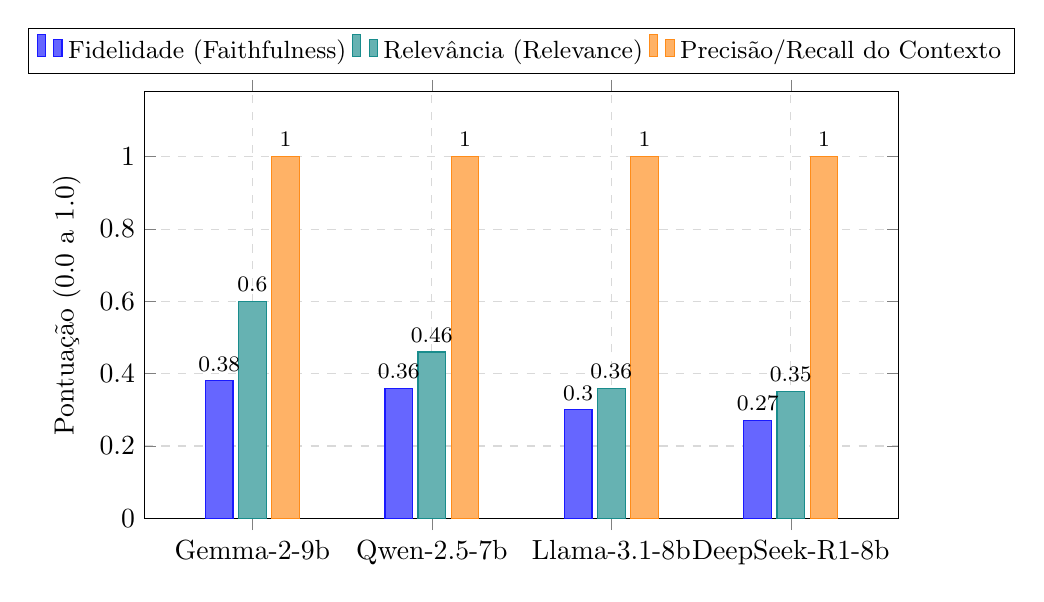
\begin{tikzpicture}
\begin{axis}[
    ybar,
    bar width=0.35cm,
    width=0.92\textwidth,
    height=7.0cm,
    enlarge x limits=0.20,
    legend style={at={(0.5,1.15)}, anchor=north, legend columns=-1, font=\small},
    ylabel={Pontuação (0.0 a 1.0)},
    symbolic x coords={Gemma-2-9b, Qwen-2.5-7b, Llama-3.1-8b, DeepSeek-R1-8b},
    xtick=data,
    nodes near coords,
    nodes near coords align={vertical},
    every node near coord/.append style={font=\footnotesize},
    ymin=0, ymax=1.18,
    grid=major,
    grid style={dashed, gray!30}
]

% Faithfulness
\addplot[fill=blue!60, draw=blue!90] coordinates {
    (Gemma-2-9b, 0.38)
    (Qwen-2.5-7b, 0.36)
    (Llama-3.1-8b, 0.30)
    (DeepSeek-R1-8b, 0.27)
};

% Answer Relevance
\addplot[fill=teal!60, draw=teal!90] coordinates {
    (Gemma-2-9b, 0.60)
    (Qwen-2.5-7b, 0.46)
    (Llama-3.1-8b, 0.36)
    (DeepSeek-R1-8b, 0.35)
};

% Context Precision / Recall
\addplot[fill=orange!60, draw=orange!90] coordinates {
    (Gemma-2-9b, 1.00)
    (Qwen-2.5-7b, 1.00)
    (Llama-3.1-8b, 1.00)
    (DeepSeek-R1-8b, 1.00)
};

\legend{Fidelidade (Faithfulness), Relevância (Relevance), Precisão/Recall do Contexto}
\end{axis}
\end{tikzpicture}
\caption{Comparativo das métricas do framework RAGAS entre as quatro arquiteturas de LLMs avaliadas.}
\label{fig:grafico_ragas}
\end{figure}
